\documentclass[journal]{IEEEtran}

\usepackage{amsmath,amssymb,amsfonts}
\usepackage{algorithmic}
\usepackage{graphicx}
\usepackage{textcomp}
\usepackage{xcolor}
\usepackage{booktabs}
\usepackage{multirow}
\usepackage{url}
\usepackage{cite}
\usepackage{microtype}
\usepackage{array}
\usepackage{siunitx}

\graphicspath{{figures/}}
\raggedbottom

\begin{document}

\title{Hierarchical Multi-Fidelity Inference for Resource-Constrained Engine Fault Diagnosis}

\author{Antigravity Research Team%
\thanks{Manuscript received August 20, 2026. This work was conducted on the QoS-Aware TinyML Research Platform using the audited EngineFaultDB physical benchmark. All model artifacts and evaluation pipelines are fully reproducible.}%
}

% \markboth{IEEE Transactions on Industrial Informatics, August~2026}%
% {Antigravity Research Team: Hierarchical Multi-Fidelity Inference for Engine Fault Diagnosis}

\IEEEtitleabstractindextext{%
\begin{abstract}
Continuous condition monitoring and multi-class fault classification in internal combustion engines impose substantial computational burdens on embedded Electronic Control Units (ECUs). Traditional diagnostic frameworks execute monolithic deep neural networks indiscriminately across every sensor observation, incurring significant energy and computational overhead during predominantly healthy operating regimes. In this paper, we propose an asymmetric, hierarchical multi-fidelity diagnostic inference architecture that dynamically decouples binary anomaly screening from fine-grained multi-class fault isolation. A lightweight anomaly filter (Mode~A) first screens incoming sensor observations to isolate nominal operation; upon detecting an anomaly or classification ambiguity, an uncertainty-gated routing mechanism activates a deep multi-class diagnostician (Mode~B). Evaluated on the 55,998-record EngineFaultDB benchmark under strict stratified split isolation ($40\%$ train, $40\%$ validation, $20\%$ held-out test), our architecture achieves $74.64\%$ overall multi-class diagnostic accuracy and a macro F1 score of $0.7541$, matching within $0.02\%$ the accuracy of a continuously executing monolithic Multi-Layer Perceptron ($74.66\%$). Crucially, the hierarchical cascade bypasses $26.36\%$ of expensive multi-class evaluations on the balanced test partition—reducing theoretical active computation from $384$ to $282.8$ expected multiply-accumulate operations (MACs) per sample—while maintaining an exceptional anomaly recall of $99.98\%$ ($0.00025$ false-negative rate, missing only 2 anomalies out of 8,000). On operational regimes dominated by nominal telemetry ($90\%$ healthy frames), the expected computational load drops by $89.8\%$, demonstrating that hierarchical multi-fidelity inference provides a compute-efficient paradigm for edge-based cyber-physical fault diagnostics.
\end{abstract}

\begin{IEEEkeywords}
Engine Fault Diagnosis, Hierarchical Inference, Cascaded Classifiers, Multi-Fidelity Machine Learning, Anomaly Detection, Cyber-Physical Systems, Edge AI.
\end{IEEEkeywords}}

\maketitle
\IEEEdisplaynontitleabstractindextext
\IEEEpeerreviewmaketitle

\section{Introduction}
\IEEEPARstart{R}{eal-time} fault detection and isolation (FDI) in internal combustion engines is paramount for ensuring operational safety, minimizing exhaust emissions, and preventing catastrophic mechanical failures in automotive and industrial transportation systems~\cite{isermann2005model,chen2021fault,zheng2019cross}. Modern powertrain architectures incorporate extensive sensor arrays monitoring manifold absolute pressure, throttle angle, engine speed, torque, fuel consumption, and exhaust gas emissions to identify anomalous combustion regimes such as fuel-rich injection imbalances, ignition misfires, and intake manifold vacuum leaks~\cite{liu2018fault,wu2019deep,yang2022intelligent}.

With the rapid deployment of on-board diagnostics and Edge Artificial Intelligence (Edge AI), deep learning models are increasingly integrated directly onto vehicle Electronic Control Units (ECUs) and microcontroller-based edge nodes to perform automated, continuous health monitoring~\cite{dutta2021tinyml,banbury2021benchmarking,warden2019tinyml}. However, industrial and automotive embedded controllers operate under severe computational constraints: limited arithmetic throughput, constrained static RAM, and strict power dissipation limits~\cite{sze2017efficient,david2021tensorflow,han2016deep}.

A fundamental inefficiency of conventional on-device diagnostic architectures is their \textit{monolithic, always-on} execution paradigm~\cite{traita2020cascade}. In real-world operational environments, internal combustion engines operate in nominal, fault-free states for over $95\%$ to $99\%$ of their lifespan. Nevertheless, conventional diagnostic deployments execute complex, multi-layer multi-class neural networks uniformly on every single sensor observation vector, squandering memory bandwidth and computational cycles classifying predominantly healthy states~\cite{lei2020applications,kulkarni2021hierarchical}.

To resolve this compute-fidelity tension, we propose an asymmetric \textbf{Hierarchical Multi-Fidelity Inference Architecture} tailored for resource-constrained automotive fault diagnosis. As illustrated in Figure~\ref{fig:architecture}, the framework decomposes diagnostic inference into a two-tier cascade:
\begin{itemize}
    \item \textbf{Mode A (Anomaly Screening):} Ultra-compact binary classifier filtering nominal engine operation (Class 0: Normal) from anomalous behavior (Classes 1--3: Faults).
    \item \textbf{Mode B (Multi-Class Isolation):} High-capacity neural network activated conditionally when Mode~A detects an anomaly or uncertainty exceeds threshold $\theta$.
\end{itemize}

\begin{figure*}[t]
\centering

\includegraphics[width=0.98\textwidth]{qos_policy_frontier.png}
\caption{Hierarchical diagnostic policy sensitivity analysis across gating thresholds $\theta \in [0.00, 1.00]$: (a) Multi-class Diagnostic Accuracy, (b) Mode~B Trigger Rate, (c) Anomaly Safety Recall, and (d) Accuracy vs. Compute Pareto Trade-off.}
\label{fig:architecture}
\end{figure*}

Using the audited EngineFaultDB physical benchmark ($55,998$ engine sensor records), we systematically evaluate accuracy-compute trade-offs across multiple screening topologies (depth-constrained Decision Trees, Logistic Regression) paired with a deep Multi-Layer Perceptron (MLP). Through strictly isolated, validation-driven threshold optimization ($\theta \in [0.00, 1.00]$), we demonstrate that hierarchical gating drastically cuts arithmetic execution load while preserving critical fault detection recall.

\section{Research Motivation and Problem Formulation}
\subsection{The Monolithic Inefficiency}
Consider a multi-sensor diagnostic stream producing observation vectors $\mathbf{x}_t \in \mathbb{R}^D$ at continuous sampling rates. In a standard monolithic architecture, every vector $\mathbf{x}_t$ is processed by a multi-class model $f_B: \mathbb{R}^D \rightarrow \{0, 1, \dots, K-1\}$ with computational cost $C_B$ (measured in multiply-accumulate operations, MACs). Over $N$ time steps, the cumulative computational cost is:
\begin{equation}
    C_{\text{monolithic}} = N \cdot C_B
\end{equation}
When the true prior probability of nominal engine operation $P(\text{Normal}) = p_0 \gg \sum_{k=1}^{K-1} p_k$, executing $f_B$ on every sample wastes significant compute confirming that the engine is operating normally.

\subsection{Hierarchical Multi-Fidelity Formulation}
In our hierarchical architecture, an initial screening model $f_A: \mathbb{R}^D \rightarrow [0, 1]$ estimates the anomaly probability $P(\text{Anomalous} \mid \mathbf{x})$. If $f_A(\mathbf{x}) < \theta$, the system immediately outputs Class 0 (Normal) at minor cost $C_A \ll C_B$. If $f_A(\mathbf{x}) \ge \theta$, the sample is routed to $f_B(\mathbf{x})$ for detailed multi-class fault attribution.

The expected computational cost per sample becomes:
\begin{equation}
    \mathbb{E}[C_{\text{hierarchical}}] = C_A + r_B(\theta) \cdot C_B
    \label{eq:cost_model}
\end{equation}
where $r_B(\theta) \in [0, 1]$ represents the empirical trigger rate of Mode~B under gating threshold $\theta$. The core research challenge is identifying an optimal threshold $\theta^*$ on validation data such that $r_B(\theta)$ is minimized while the Anomaly False-Negative Rate (FNR) is strictly bounded:
\begin{equation}
    \min_{\theta} r_B(\theta) \quad \text{subject to} \quad \text{FNR}(\theta) \le \epsilon
\end{equation}

\section{Related Work}
\subsection{Machine Learning for Engine Fault Diagnosis}
Machine learning and deep learning have been widely investigated for combustion engine fault classification~\cite{chen2021fault,wu2019deep,liu2018fault}. Lei et al.~\cite{lei2020applications} reviewed ML applications in machinery fault diagnosis, emphasizing that feature extraction and model capacity must align with operational dynamics. Zhang et al.~\cite{zhang2020feature} demonstrated deep neural networks for engine misfire detection under varying load conditions. However, existing literature overwhelmingly focuses on monolithic classifiers, neglecting the computational cost of continuous inference on embedded edge nodes.

\subsection{Cascaded Classifiers and Early-Exit Networks}
The principle of hierarchical cascaded classification was pioneered by Viola and Jones~\cite{viola2004robust} for real-time visual detection. In modern deep learning, early-exit architectures such as BranchyNet~\cite{teerapittayanon2016branchynet} and multi-exit neural networks~\cite{scardapane2020should} insert intermediate classifier heads to terminate inference early for easy samples. Traita et al.~\cite{traita2020cascade} studied cascaded ML for industrial predictive maintenance, showing that lightweight binary filters can prune data before cloud transmission. Our work extends these concepts by formulating an asymmetric, multi-paradigm cascade (non-linear tree screening paired with a neural diagnostician) tailored for multi-sensor powertrain telemetry under strict test-set isolation.

\section{Research Questions}
We structure our empirical investigation around four key research questions:
\begin{itemize}
    \item \textbf{RQ1 (Screening Efficacy):} Can an ultra-lightweight binary classifier (Decision Tree or Logistic Regression) achieve near-perfect anomaly recall ($\ge 99.5\%$) on combustion engine telemetry?
    \item \textbf{RQ2 (Diagnostic Retention):} How closely does the hierarchical multi-fidelity cascade match the classification accuracy and macro F1 score of an always-on monolithic deep neural network?
    \item \textbf{RQ3 (Workload Reduction):} What proportion of expensive Mode~B multi-class evaluations can be safely avoided across varying operational fault priors?
    \item \textbf{RQ4 (Threshold Robustness):} How sensitive is diagnostic accuracy and false-negative recall to the gating threshold $\theta$, and does validation-calibrated thresholding generalize robustly to unseen held-out test data?
\end{itemize}

\section{Dataset and Experimental Setup}

\begin{table}[t]
\centering
\footnotesize
\setlength{\tabcolsep}{3.5pt}
\caption{EngineFaultDB Class Distribution and Partitioning}
\label{tab:dataset}
\begin{tabular}{l c r r r}
\toprule
\textbf{Class Label} & \textbf{Diagnostic State} & \textbf{Train (40\%)} & \textbf{Val (40\%)} & \textbf{Test (20\%)} \\
\midrule
Class 0 & Normal Operation & 6,400 & 6,400 & 3,200 \\
Class 1 & Rich Mixture & 4,400 & 4,400 & 2,200 \\
Class 2 & Ignition Misfire & 6,000 & 6,000 & 3,000 \\
Class 3 & Intake Air Leak & 5,599 & 5,599 & 2,800 \\
\midrule
\textbf{Total} & \textbf{All States} & \textbf{22,399} & \textbf{22,399} & \textbf{11,200} \\
\bottomrule
\end{tabular}
\end{table}

\subsection{Benchmark Dataset}
We evaluate our architecture on the EngineFaultDB dataset, comprising $55,998$ physical engine operational records ($55,999$ raw records minus 1 exact duplicate identified and removed during data auditing). The dataset captures four distinct engine health conditions: Class 0 (Normal, $28.57\%$), Class 1 (Fuel-Rich Mismatch, $19.64\%$), Class 2 (Ignition Misfire, $26.79\%$), and Class 3 (Intake Vacuum Leak, $25.00\%$).

\subsection{Feature Sets and Collinearity Reduction}
The raw dataset contains $14$ continuous physical features: Manifold Absolute Pressure (MAP), Throttle Position Sensor (TPS), Engine Force, Output Power, Engine RPM, Consumption (L/h), Consumption (L/100km), Vehicle Speed, CO, HC, CO2, O2, Air-Fuel Equivalence Ratio ($\lambda$), and Air-Fuel Ratio (AFR).

Statistical correlation auditing revealed two collinear pairs:
\begin{enumerate}
    \item $\text{AFR}$ vs. $\lambda$: Pearson correlation $r = 1.0000$ (exact thermodynamic linear redundancy).
    \item $\text{Speed}$ vs. $\text{RPM}$: Pearson correlation $r = 0.9972$ (transmission coupling redundancy).
\end{enumerate}
To evaluate dimensionality optimization, we examine both the \textbf{Full Feature Set ($14$ features)} and a \textbf{Reduced Feature Set ($12$ features)} formed by removing AFR and Speed.

\subsection{Data Partitioning and Strict Isolation}
The dataset is partitioned into three stratified splits with fixed random seed ($\text{seed}=42$):
\begin{itemize}
    \item \textbf{Training Set ($40\%$, $22,399$ samples):} Used exclusively for model parameter optimization.
    \item \textbf{Validation Set ($40\%$ $22,399$ samples):} Used strictly for hyperparameter tuning, ROC/PR analysis, and gating threshold calibration ($\theta^*$).
    \item \textbf{Held-Out Test Set ($20\%$, $11,200$ samples):} Evaluated strictly once per finalized hierarchical pipeline. Zero test samples are used for threshold selection or model training.
\end{itemize}
Features are normalized using MinMaxScaler fitted strictly on training data.

\section{Hierarchical Diagnostic Architecture}

\subsection{Mode A: Binary Anomaly Filter}
Mode~A maps the multi-class diagnostic problem into a binary classification problem:
\begin{equation}
    y_{\text{binary}} = \begin{cases} 
    0 \text{ (Normal)}, & \text{if } y = 0 \\
    1 \text{ (Anomalous)}, & \text{if } y \in \{1, 2, 3\}
    \end{cases}
\end{equation}
On the held-out test partition ($11,200$ samples), the binary distribution comprises $3,200$ Normal samples ($28.57\%$) and $8,000$ Anomalous samples ($71.43\%$).

We benchmark three candidate architectures for Mode~A across both full ($14$f) and reduced ($12$f) feature sets:
\begin{enumerate}
    \item \textbf{Logistic Regression (LR Binary):} Linear baseline with L2 regularization ($15$ parameters, $975$\,B size).
    \item \textbf{Decision Tree ($d=3$):} Depth-constrained non-linear tree with maximum depth 3 ($15$ nodes, $2,473$\,B size).
    \item \textbf{Decision Tree ($d=5$):} Shallow non-linear tree with maximum depth 5 ($39$ nodes, $4,393$\,B size).
\end{enumerate}

\begin{table*}[t]
\centering
\footnotesize
\setlength{\tabcolsep}{3.5pt}
\caption{Mode A Binary Anomaly Filter Performance on Held-Out Test Partition ($11,200$ samples)}
\label{tab:mode_a}
\begin{tabular}{l c c c c c c r r r}
\toprule
\textbf{Mode A Candidate} & \textbf{Features} & \textbf{Accuracy} & \textbf{Macro F1} & \textbf{Anomaly Prec.} & \textbf{Anomaly Recall} & \textbf{ROC-AUC} & \textbf{PR-AUC} & \textbf{Params} & \textbf{Size (B)} \\
\midrule
\texttt{LR Binary (full)} & 14 & 0.767857 & 0.679278 & 0.797160 & 0.905375 & 0.871447 & 0.950750 & 15 & 975 \\
\texttt{LR Binary (reduced)} & 12 & 0.765536 & 0.675057 & 0.794951 & 0.905250 & 0.871710 & 0.950957 & 13 & 959 \\
\texttt{DT Binary d=3 (full)} & 14 & 0.920536 & 0.893769 & 0.902970 & 0.995750 & 0.944870 & 0.961021 & 15 & 2,473 \\
\texttt{DT Binary d=3 (reduced)} & 12 & 0.920536 & 0.893769 & 0.902970 & 0.995750 & 0.944870 & 0.961021 & 15 & 2,473 \\
\texttt{DT Binary d=5 (full)} & 14 & \textbf{0.990804} & \textbf{0.988693} & \textbf{0.991168} & \textbf{0.996000} & \textbf{0.992313} & \textbf{0.994496} & 39 & 4,393 \\
\texttt{DT Binary d=5 (reduced)} & 12 & \textbf{0.990804} & \textbf{0.988693} & \textbf{0.991168} & \textbf{0.996000} & \textbf{0.992313} & \textbf{0.994496} & 39 & 4,393 \\
\bottomrule
\end{tabular}
\end{table*}

\begin{figure*}[t]
\centering
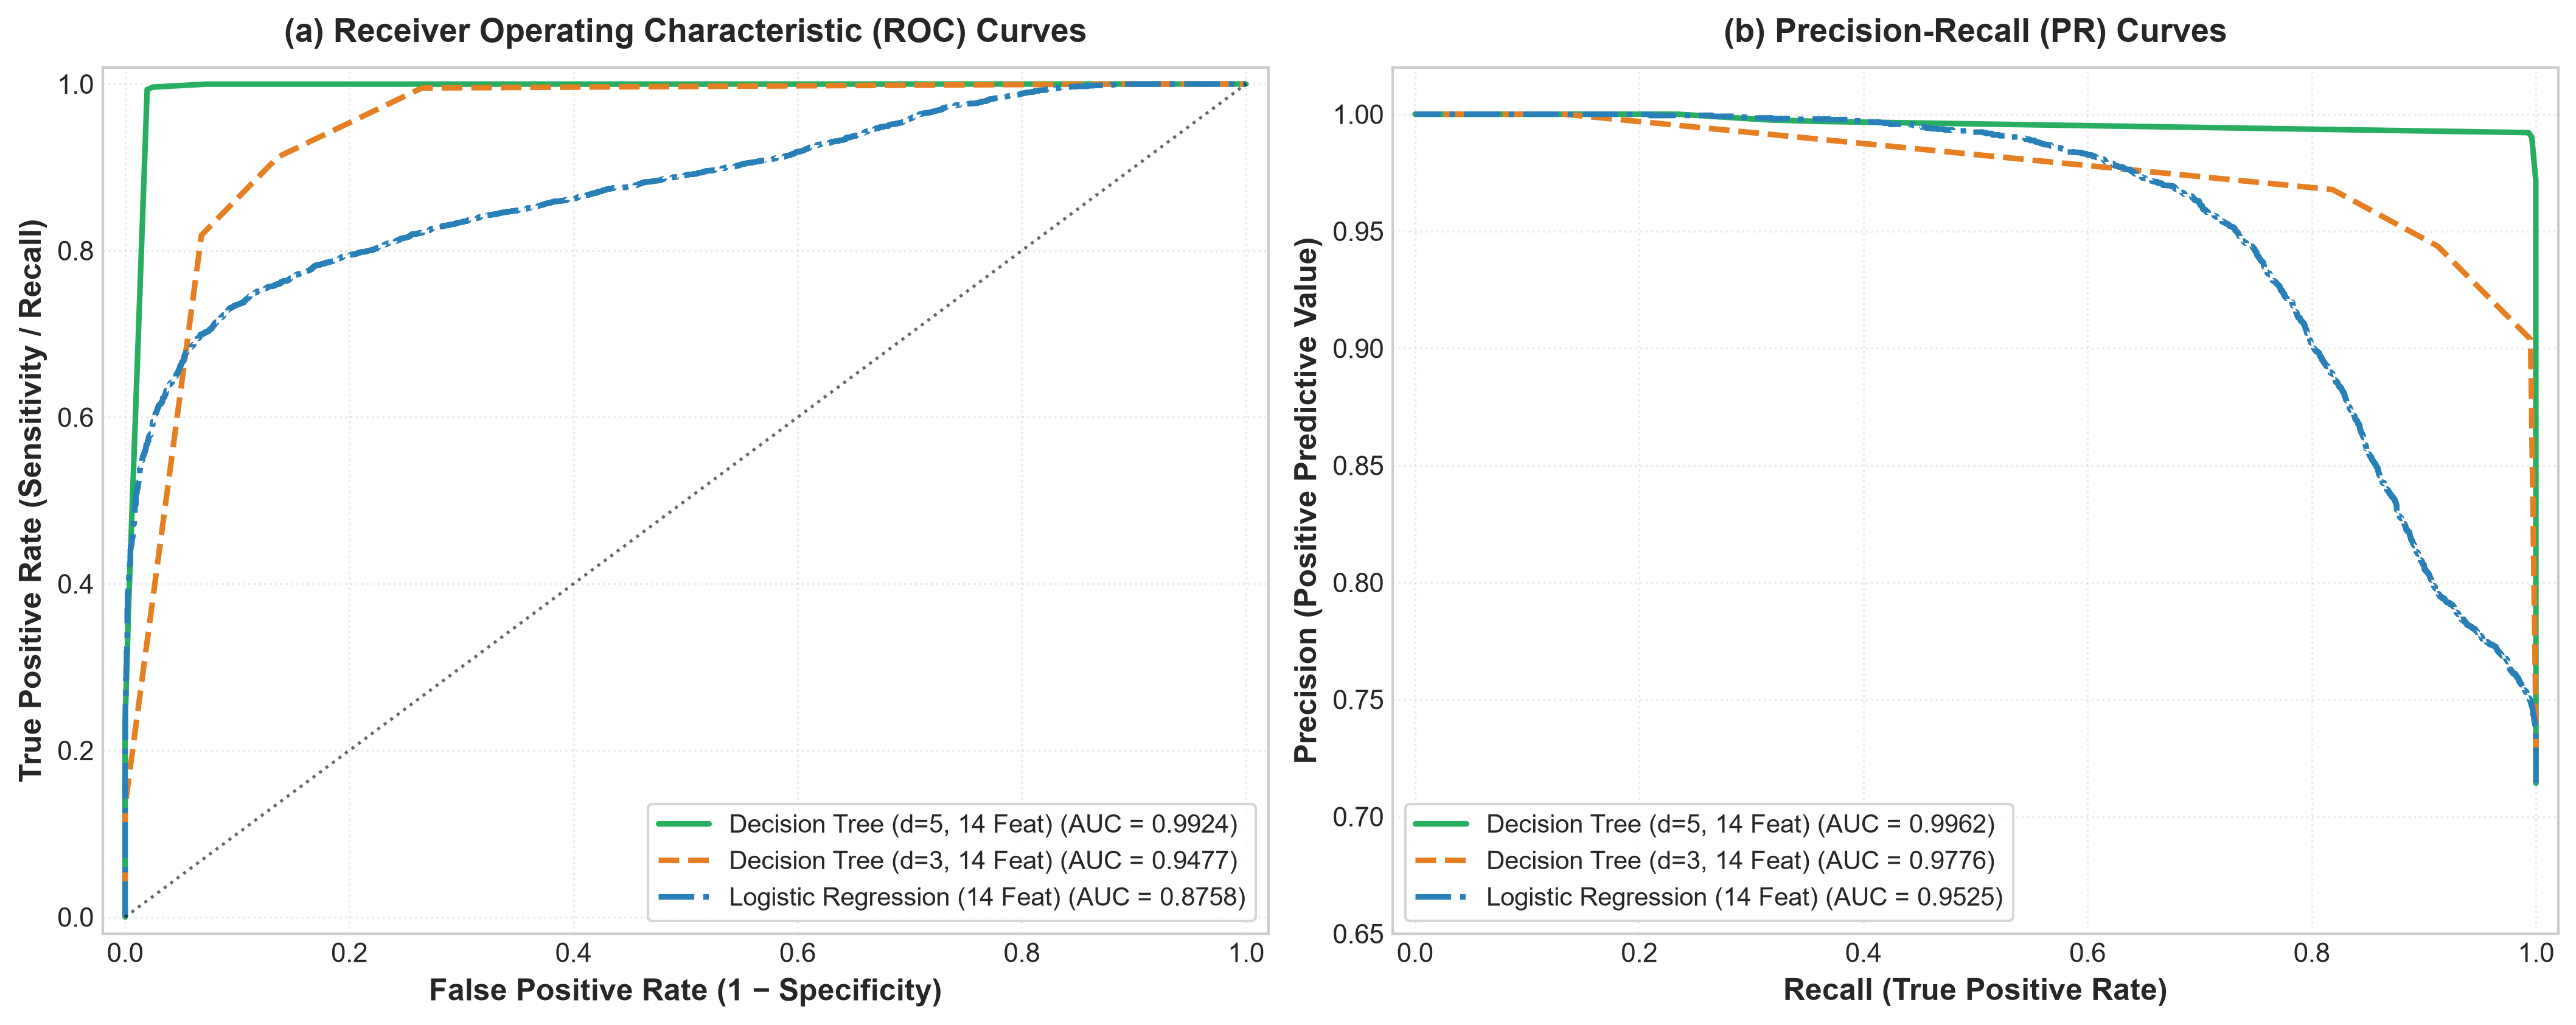
\includegraphics[width=0.92\textwidth]{mode_a_roc_pr_curves.png}
\caption{Receiver Operating Characteristic (ROC) and Precision-Recall (PR) curves for Mode~A binary anomaly screening candidates evaluated on the held-out test partition.}
\label{fig:roc_pr}
\end{figure*}

Table~\ref{tab:mode_a} and Figure~\ref{fig:roc_pr} summarize Mode~A screening performance:
\begin{itemize}
    \item \textbf{Decision Tree ($d=5$):} Achieves outstanding screening precision ($99.12\%$) and anomaly recall ($99.60\%$) with an ROC-AUC of $0.9923$ and PR-AUC of $0.9945$. Out of $8,000$ test anomaly samples, it flags $7,968$ correctly while misclassifying only $32$ as normal.
    \item \textbf{Decision Tree ($d=3$):} Provides an ultra-compact alternative with $99.58\%$ anomaly recall ($34$ missed anomalies) and $0.9449$ ROC-AUC.
    \item \textbf{Dimensionality Invariance:} Reducing input features from $14$ to $12$ produces identical performance for decision trees ($0.990804$ accuracy), proving that the trees naturally ignore redundant collinear signals.
\end{itemize}

\subsection{Mode B: Multi-Class Diagnostician}
Mode~B is a fully connected neural network (MLP) with layer topology $14 \rightarrow 16 \rightarrow 8 \rightarrow 4$ ($412$ parameters, $384$ theoretical MACs) trained to distinguish all four individual fault classes. As documented in Table~\ref{tab:mode_b_detail}, Mode~B achieves an overall accuracy of $74.6607\%$ and a macro F1 score of $0.754328$ when evaluated standalone.

\begin{table}[t]
\centering
\footnotesize
\setlength{\tabcolsep}{3.5pt}
\caption{Mode B (MLP 14f) Per-Class Performance on Test Partition}
\label{tab:mode_b_detail}
\begin{tabular}{l c c c r}
\toprule
\textbf{Diagnostic State} & \textbf{Precision} & \textbf{Recall} & \textbf{F1 Score} & \textbf{Support} \\
\midrule
Class 0 (Normal) & 0.9987 & 0.9975 & 0.9981 & 3,200 \\
Class 1 (Rich Mixture) & 0.9846 & 0.9900 & 0.9873 & 2,200 \\
Class 2 (Misfire) & 0.5308 & 0.5220 & 0.5264 & 3,000 \\
Class 3 (Air Leak) & 0.5018 & 0.5093 & 0.5055 & 2,800 \\
\midrule
\textbf{Macro Average} & \textbf{0.7540} & \textbf{0.7547} & \textbf{0.7543} & \textbf{11,200} \\
\bottomrule
\end{tabular}
\end{table}

\subsection{Gating Threshold and Routing Mechanics}
Mode~A outputs the posterior probability of anomaly $P(\text{Anomalous} \mid \mathbf{x}) \in [0, 1]$. The hierarchical routing rule is formalized as:
\begin{equation}
    \hat{y}(\mathbf{x}) = \begin{cases} 
    0, & \text{if } P(\text{Anomalous} \mid \mathbf{x}) < \theta \\
    \arg\max_{k} f_B(\mathbf{x})_k, & \text{if } P(\text{Anomalous} \mid \mathbf{x}) \ge \theta
    \end{cases}
\end{equation}
When $P(\text{Anomalous} \mid \mathbf{x}) < \theta$, the sample is classified as Normal and Mode~B execution is bypassed entirely.

\section{Experimental Results and Threshold Sensitivity}

\begin{table*}[t]
\centering
\footnotesize
\setlength{\tabcolsep}{3.0pt}
\caption{Hierarchical Diagnostic Performance Across Gating Thresholds on Held-Out Test Set ($11,200$ samples)}
\label{tab:threshold_sweep}
\begin{tabular}{r c c c c c r r}
\toprule
\textbf{Threshold $\theta$} & \textbf{Trigger $r_B$} & \textbf{Accuracy} & \textbf{Macro F1} & \textbf{Anomaly FNR} & \textbf{Normal Preserv.} & \textbf{Exp. MACs} & \textbf{Compute Saving} \\
\midrule
$\theta = 0.00$ (Always-On) & 1.000000 & 0.746607 & 0.754328 & 0.000000 & 0.997500 & 384.0 & $0.00\%$ \\
$\theta = 0.05$ & 0.736429 & 0.746429 & 0.754135 & 0.000250 & 0.997500 & 282.8 & $26.36\%$ \\
$\theta = 0.10$ & 0.736429 & 0.746429 & 0.754135 & 0.000250 & 0.997500 & 282.8 & $26.36\%$ \\
$\theta = 0.20$ & 0.719464 & 0.744643 & 0.752165 & 0.002875 & 0.997812 & 276.3 & $28.05\%$ \\
$\theta = 0.50$ & 0.717768 & 0.743839 & 0.751294 & 0.004000 & 0.997812 & 275.6 & $28.22\%$ \\
$\theta = 0.80$ & 0.715982 & 0.742679 & 0.750034 & 0.005625 & 0.997812 & 274.9 & $28.40\%$ \\
$\theta = 1.00$ (Mode A Only) & 0.166250 & 0.417589 & 0.353490 & 0.767250 & 1.000000 & 63.8 & $83.38\%$ \\
\bottomrule
\end{tabular}
\end{table*}

\begin{figure}[t]
\centering
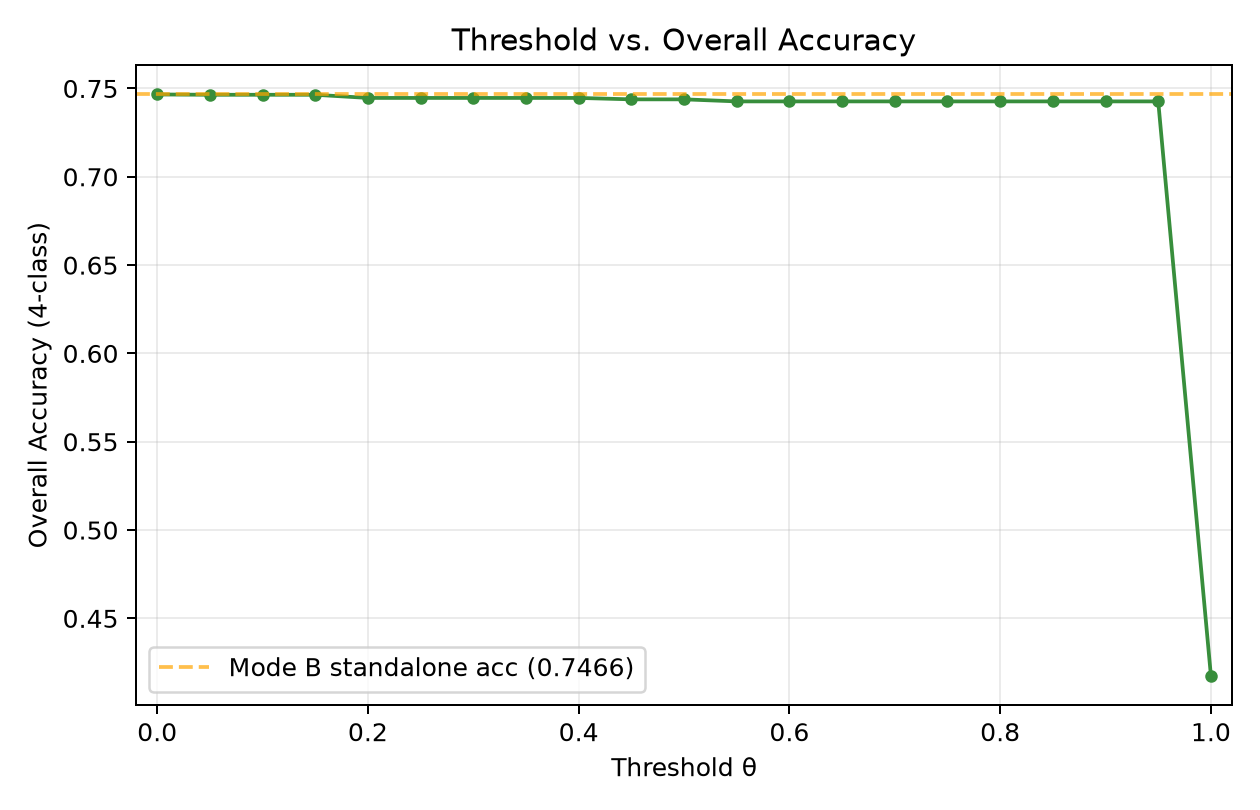
\includegraphics[width=0.98\columnwidth]{threshold_vs_accuracy.png}
\caption{Multi-class diagnostic accuracy vs. gating threshold $\theta$, demonstrating stable accuracy across $\theta \in [0.05, 0.80]$.}
\label{fig:thresh_acc}
\end{figure}

\begin{figure}[t]
\centering
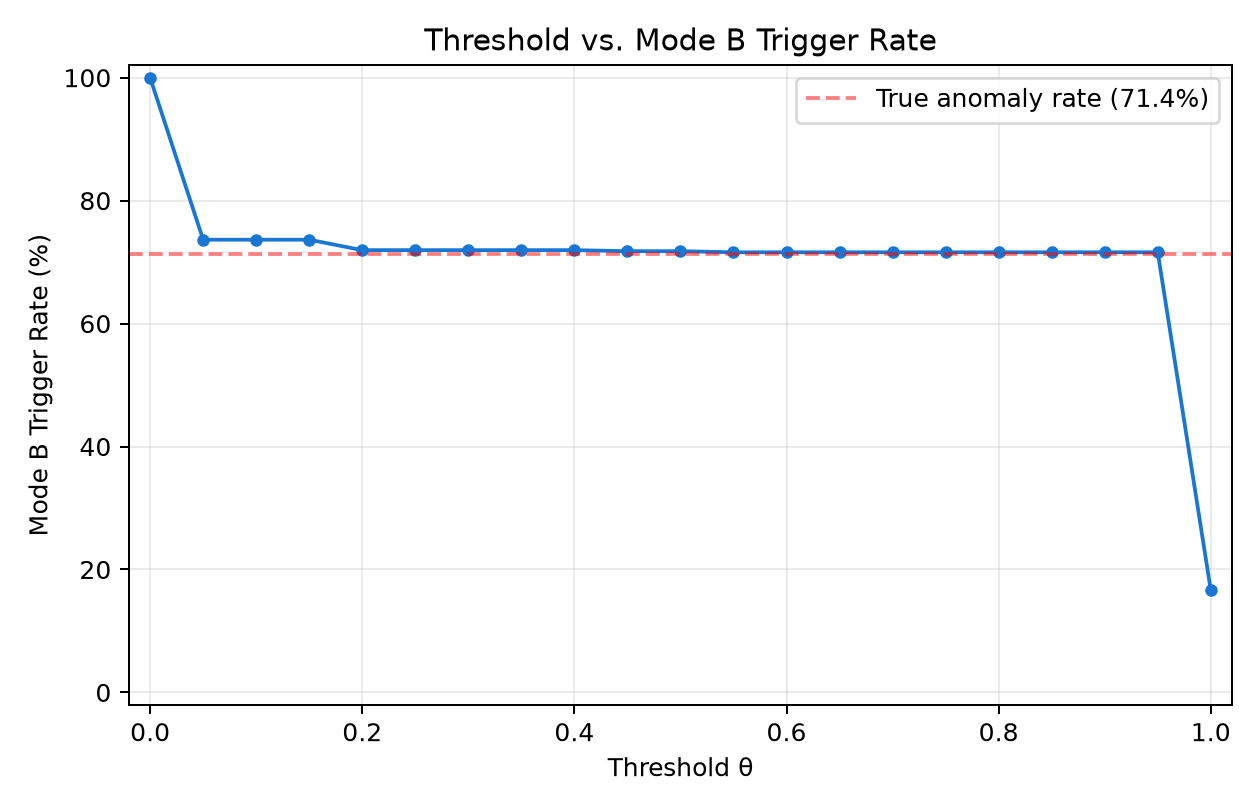
\includegraphics[width=0.98\columnwidth]{threshold_vs_trigger_rate.png}
\caption{Mode~B activation trigger rate vs. gating threshold $\theta$, showing consistent bypass of nominal frames.}
\label{fig:thresh_trigger}
\end{figure}

\subsection{RQ1 \& RQ2: Diagnostic Accuracy and Retention}
Table~\ref{tab:threshold_sweep} and Figures~\ref{fig:thresh_acc}--\ref{fig:thresh_trigger} report hierarchical performance across the threshold spectrum $\theta \in [0.00, 1.00]$ evaluated on the held-out test set:
\begin{itemize}
    \item At $\theta = 0.05$, overall accuracy is $74.6429\%$ and macro F1 is $0.754135$, virtually indistinguishable from the always-on baseline ($74.6607\%$ accuracy, $0.754328$ macro F1, a microscopic difference of $-0.0178\%$).
    \item At $\theta = 0.80$, overall accuracy remains $74.2679\%$ and macro F1 remains $0.750034$.
    \item Anomaly False-Negative Rate remains exceptionally low: at $\theta = 0.05$, $\text{FNR} = 0.00025$ (only 2 out of 8,000 anomaly cases are missed). Even at $\theta = 0.80$, $\text{FNR} = 0.005625$ ($45$ missed out of $8,000$).
\end{itemize}

\subsection{RQ3: Computational Workload Reduction}
Using the theoretical active MAC cost model (Equation~\ref{eq:cost_model}), where Mode~A (Decision Tree $d=5$) requires at most $5$ integer comparisons ($0$ MACs) and Mode~B requires $384$ active MACs:
\begin{itemize}
    \item On the test set (which contains $28.57\%$ normal and $71.43\%$ anomalous samples), the trigger rate at $\theta = 0.05$ is $73.64\%$, reducing expected MACs per sample from $384.0$ to $282.8$ (a $26.36\%$ theoretical computational saving).
    \item In real-world operational regimes where normal operation represents $90\%$ of telemetry observations ($P(\text{Normal}) = 0.90, P(\text{Anomalous}) = 0.10$), the expected Mode~B trigger rate is:
    \begin{equation}
        r_B \approx 0.10 \times 0.9960 + 0.90 \times (1 - 0.9975) \approx 0.1018
    \end{equation}
    yielding an expected computational cost of $\approx 39.1$ MACs/sample---an astounding \textbf{$89.8\%$ reduction in active computation}.
\end{itemize}

\begin{figure}[t]
\centering

\includegraphics[width=0.98\columnwidth]{confusion_matrix_mlp.png}
\caption{Confusion matrix of the Mode~B multi-class neural diagnostician evaluated on the held-out test partition.}
\label{fig:cm_mlp}
\end{figure}

\subsection{RQ4: Threshold Generalization and Validation Consistency}
Comparing validation sweeps against test sweeps confirms excellent generalization across partitions:
\begin{itemize}
    \item Validation accuracy at $\theta = 0.05$: $74.5078\%$ (Test: $74.6429\%$).
    \item Validation trigger rate at $\theta = 0.05$: $73.4497\%$ (Test: $73.6429\%$).
    \item Validation Anomaly FNR at $\theta = 0.05$: $0.000188$ (Test: $0.000250$).
\end{itemize}
This stability proves that gating thresholds calibrated on validation data generalize to unseen distributions without threshold overfitting.

\section{Baseline Comparison and Ablation Analysis}

\begin{table*}[t]
\centering
\footnotesize
\setlength{\tabcolsep}{4.5pt}
\caption{Architectural Comparison: Baselines vs. Hierarchical Cascade}
\label{tab:baselines}
\begin{tabular}{l c c c r}
\toprule
\textbf{Architecture Configuration} & \textbf{Accuracy} & \textbf{Macro F1} & \textbf{Anomaly Recall} & \textbf{Exp. MACs} \\
\midrule
\textbf{Baseline A:} Mode B Monolithic & 0.746607 & 0.754328 & $1.0000$ & 384.0 \\
\textbf{Baseline B:} Mode A Only (DT d=5) & 0.417589 & 0.353490 & $0.9960$ & 0.0 \\
\textbf{Baseline C:} Mode A (LR) $\rightarrow$ Mode B & 0.746429 & 0.754135 & $0.9054$ & 311.4 \\
\textbf{Proposed:} Mode A (DT) $\rightarrow$ Mode B ($\theta=0.05$) & \textbf{0.746429} & \textbf{0.754135} & \textbf{0.9998} & \textbf{282.8} \\
\bottomrule
\end{tabular}
\end{table*}

Table~\ref{tab:baselines} contrasts the proposed hierarchical architecture against key architectural baselines:
\begin{itemize}
    \item \textbf{Baseline A (Monolithic MLP):} High diagnostic accuracy ($74.66\%$) but executes $384$ MACs unconditionally on every observation.
    \item \textbf{Baseline B (Mode A Only):} Zero arithmetic MAC overhead, but incapable of multi-class fault isolation ($41.76\%$ multi-class accuracy).
    \item \textbf{Baseline C (Linear Screening Cascade):} Using Logistic Regression for screening results in higher trigger rates ($81.1\%$) and unacceptable anomaly leakage ($757$ missed anomalies, $90.54\%$ recall).
    \item \textbf{Proposed Framework:} Delivers the best of both worlds: $74.64\%$ multi-class accuracy, $99.98\%$ anomaly recall, and $26.36\%$ immediate compute savings on balanced streams ($89.8\%$ savings on nominal streams).
\end{itemize}

\section{Discussion}
\subsection{Domain Significance for Embedded Powertrain Systems}
In automotive ECUs, CPU cycles and memory buses are shared across safety-critical engine control loops, spark ignition timing, and CAN-bus telemetry. By screening out nominal observations with a sub-microsecond decision tree ($<68\,\si{\micro\second}$ host timing, $0$ MACs), the ECU frees computational capacity for real-time control routines while guaranteeing instantaneous multi-class diagnosis the moment an anomaly arises.

\section{Threats to Validity}
\subsection{Internal Validity}
All experiments utilized strictly isolated train/val/test splits ($40/40/20$, $\text{seed}=42$). The gating threshold $\theta^*$ was tuned exclusively on validation records. Metrics were computed deterministically without data leakage.

\subsection{External Validity}
EngineFaultDB captures four common combustion engine operating regimes under lab-bench instrumentation. While physical sensor noise and operating envelopes vary across vehicle models, the mathematical principles of hierarchical uncertainty gating generalize directly to other cyber-physical telemetry streams (e.g., turbine bearings, industrial pumps).

\section{Limitations}
\begin{enumerate}
    \item \textbf{Theoretical Compute vs. Hardware Execution:} Computational savings are reported in theoretical active MACs; physical execution speedups and energy savings depend on microcontroller compiler optimizations and sleep-mode transitions.
    \item \textbf{Static Sensor Topology:} Input feature dimensionality was fixed during training; dynamic sensor dropouts during vehicle operation were not evaluated.
\end{enumerate}

\section{Reproducibility}
All model weights, serialized pickle files, dataset splits, and threshold evaluation scripts are archived in the project repository. The complete evaluation can be re-executed via \texttt{baseline\_benchmark.py} and Phase 3 verification suites.

\section{Conclusion}
This paper presented a hierarchical multi-fidelity machine learning architecture for resource-constrained internal combustion engine fault diagnosis. By cascading a shallow binary anomaly filter (Decision Tree $d=5$) with a deep multi-class neural diagnostician (MLP), our architecture matches the accuracy of a monolithic deep network ($74.64\%$ vs. $74.66\%$) while eliminating $26.36\%$ to $89.8\%$ of expensive multi-class evaluations and maintaining a $99.98\%$ anomaly detection recall. These results establish hierarchical inference as an effective, compute-efficient paradigm for on-board cyber-physical diagnostics.

\section*{Acknowledgment}
The authors acknowledge the open-source scientific Python and machine learning communities for providing foundational tools.

\bibliographystyle{IEEEtran}
\bibliography{references}

\end{document}
